\documentclass[a4paper,12pt]{article}[abntex2]
\bibliographystyle{abntex2-alf}
\usepackage{siunitx} % Fornece suporte para a tipografia de unidades do Sistema Internacional e formatação de números
\usepackage{booktabs} % Melhora a qualidade das tabelas
\usepackage{tabularx} % Permite tabelas com larguras de colunas ajustáveis
\usepackage{graphicx} % Suporte para inclusão de imagens
\usepackage{newtxtext} % Substitui a fonte padrão pela Times Roman
\usepackage{ragged2e} % Justificação de texto melhorada
\usepackage{setspace} % Controle do espaçamento entre linhas
\usepackage[a4paper, left=3.0cm, top=3.0cm, bottom=2.0cm, righ=2.0cm]{geometry} % Personalização das margens do documento
\usepackage{lipsum} % Geração de texto dummy 'Lorem Ipsum'
\usepackage{fancyhdr} % Customização de cabeçalhos e rodapés
\usepackage{titlesec} % Personalização dos títulos de seções
\usepackage[portuguese]{babel} % Adaptação para o português (nomes e hifenização
\usepackage{hyperref} % Suporte a hiperlinks
\usepackage{indentfirst} % Indentação do primeiro parágrafo das seções
\sisetup{
  output-decimal-marker = {,},
  inter-unit-product = \ensuremath{{}\cdot{}},
  per-mode = symbol
}
\DeclareSIUnit{\real}{R\$}
\newcommand{\real}[1]{R\$#1}
\usepackage{float} % Melhor controle sobre o posicionamento de figuras e tabelas
\usepackage{footnotehyper} % Notas de rodapé clicáveis em combinação com hyperref
\hypersetup{
    colorlinks=true,
    linkcolor=black,
    filecolor=magenta,      
    urlcolor=cyan,
    citecolor=black,        
    pdfborder={0 0 0},
}
\usepackage[normalem]{ulem} % Permite o uso de diferentes tipos de sublinhados sem alterar o \emph{}
\makeatletter
\def\@pdfborder{0 0 0} % Remove a borda dos links
\def\@pdfborderstyle{/S/U/W 1} % Estilo da borda dos links
\makeatother
\onehalfspacing

\begin{document}

\begin{titlepage}
    \centering
    \vspace*{1cm}
    \Large\textbf{INSPER – INSTITUTO DE ENSINO E PESQUISA}\\
    \Large \textbf{ECONOMIA}\\
    \vspace{1.5cm}
    \Large\textbf{Atividade Prática Superviosionada III}\\
    \textbf{Macroeconomia Internacional}\\
    \vspace{1.5cm}
    Prof. Gino Olivares\\
    Prof. Auxiliar Victor Dias \\
    \vfill
    \normalsize
    Fabrizio Antonini Ripoli, \href{mailto:fabrizioar@al.insper.edu.br}{fabrizioar@al.insper.edu.br}\\
    Hicham Munir Tayfour, \href{mailto:hichamt@al.insper.edu.br}{hichamt@al.insper.edu.br}\\
    4º Período - Economia B\\
    \vfill
    São Paulo\\
    Abril/2024
\end{titlepage}

\newpage
\tableofcontents
\thispagestyle{empty} % This command removes the page number from the table of contents page
\newpage
\setcounter{page}{1} % This command sets the page number to start from this page
\justify
\onehalfspacing

\pagestyle{fancy}
\fancyhf{}
\rhead{\thepage}

\section{\textbf{Questão 1}}
\subsection{\textbf{Letra A}}

\begin{figure}[H]
    \centering
    \caption{Preços Totalmente Flexíveis} 
    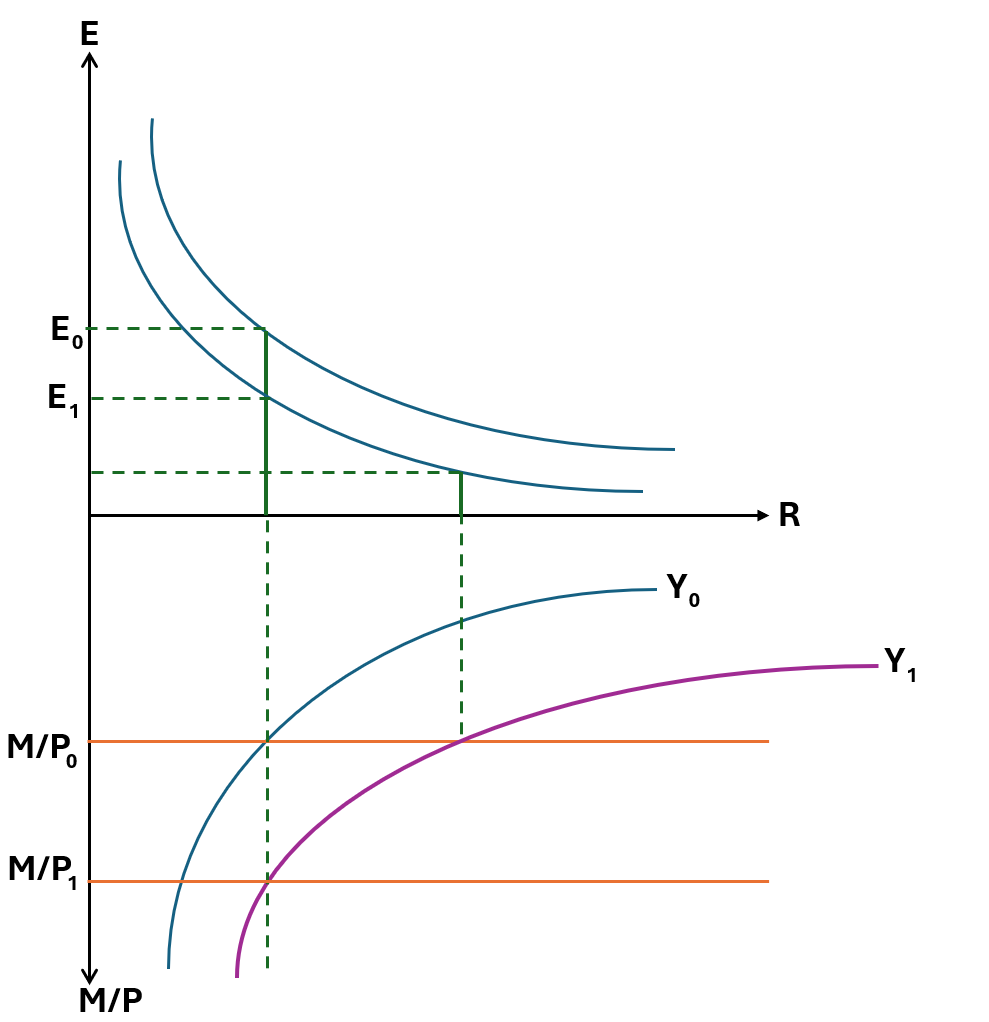
\includegraphics[width=0.75\textwidth]{Macroeconomia Internacional/APS 3 Macro Int/Preços Totalmente Flexíveis.png}
    \label{fig:preçoflexível}
    
    \footnotesize{Fonte: Elaborado pelos autores.}
    \end{figure}

O aumento da produtividade causa um choque positivo na demanda por moeda, fazendo com que  a curva se desloque positivamente, saindo de $Y_0$ para $Y_1$. Como os preços são totalmente flexíveis eles diminuirão de modo a se ajustar ao novo nível de demanda. Por consequência dos ajustes de preços, a oferta real de moeda aumenta para $M/P_1$, fazendo possível a estabilidade da taxa de juros nesse choque (virtualmente o juros aumentaria e depois diminuiria para seu nível inicial mas levando em conta preços completamente flexíveis, a resposta da oferta de moeda seria instantânea). Assim, aumentando a atividade permanentemente, por mais que não haja mudança no câmbio a partir dos juros, a expectativa de câmbio, por conta do aquecimento da economia, aumentará, mudando o valor do câmbio hoje para $E_1$.

\subsection{\textbf{Letra B}}
\begin{figure}[H]
    \centering
    \caption{Preços Fixos no Curto Prazo} 
    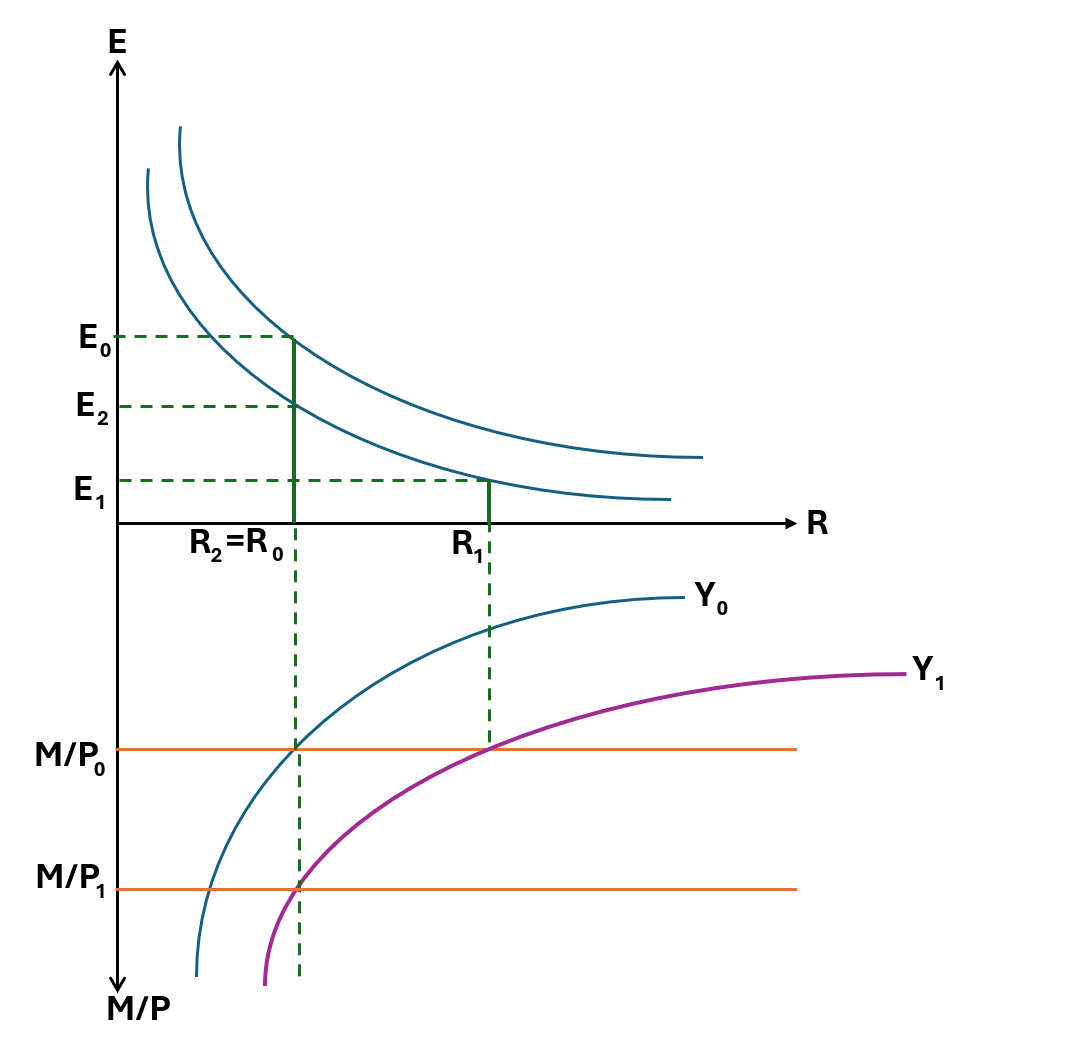
\includegraphics[width=0.75\textwidth]{Macroeconomia Internacional/APS 3 Macro Int/Preços Fixos no Curto Prazo.png}
    \label{fig:preçofixo}
    
    \footnotesize{Fonte: Elaborado pelos autores.}
    \end{figure}

O aumento da produtividade causa um choque positivo na demanda por moeda, fazendo com que  a curva se desloque positivamente, saindo de $Y_0$ para $Y_1$. Como os preços estão fixos , devido ao fato de estarmos no curto prazo, a taxa de juros irá subir , saindo de $R_0$ para $R_1$. Devido ao aumento permanente da produtividade o novo câmbio esperado vai apreciar em relação ao inicial, fazendo com que a curva de câmbio se desloque para baixo, e devido ao novo juros de curto prazo e a nova curva de câmbio, o câmbio de equilíbrio de curto prazo seria $E_1$.

No longo prazo, os preços irão se ajustar, saindo de $P_0$ para $P_1$, onde $P_1 < P_0$ , essa redução dos preços, dada a oferta monetária constante, faz com que a oferta real de moeda aumente. Fazendo com que a curva se desloque positivamente, saindo de $M/P_0$ para $M/P_1$, esta nova curva , junto da curva $Y_1$, faz com que novo juros de equilíbrio $R_2$ seja igual ao de antes do choque positivo de produtividade , $R_0$. Dado o novo juros de equilíbrio ($R_2$), o novo câmbio de equilíbrio estará depreciado em relação ao $E_1$ , resultando $E_2$, mas estará apreciado em relação ao câmbio de antes do choque ($E_0$) . 

\section{\textbf{Questão 2}}
\begin{figure}[H]
    \centering
    \caption{Figura sobre CPI e PPI} 
    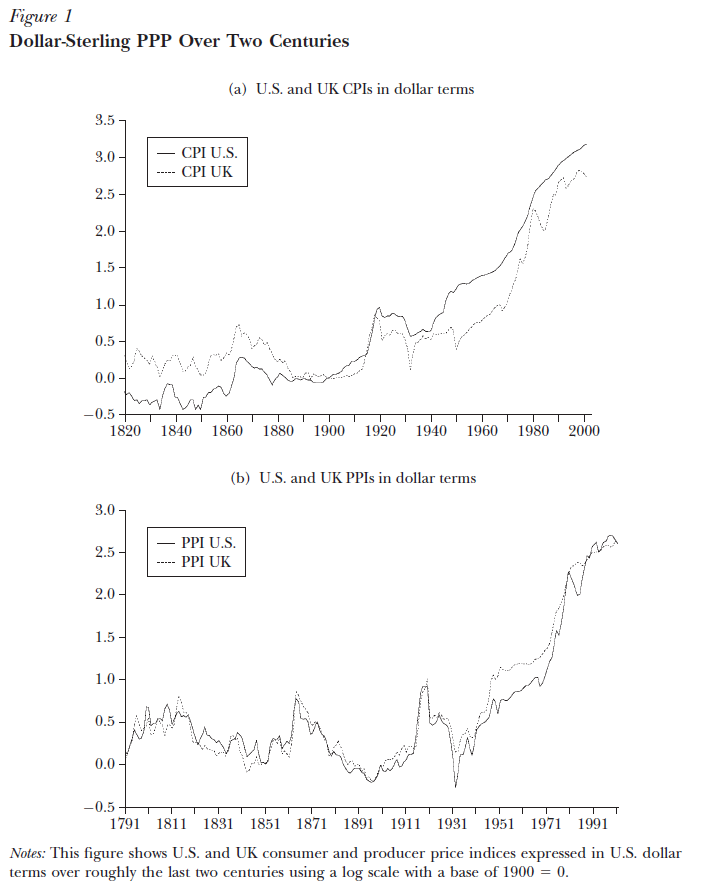
\includegraphics[width=0.75\textwidth]{Macroeconomia Internacional/APS 3 Macro Int/CPI & PPI.png}
    \label{fig:cpippi}
    
    \footnotesize{Fonte: Retirada do artigo Taylor & Taylor.}
    \end{figure}
    
A Figura~\ref{fig:cpippi}. preços ao produtor (PPI) dos EUA e do Reino Unido ao longo de um longo período histórico. Esses índices são ajustados pela taxa de câmbio, permitindo comparar a evolução dos preços relativos ajustados pela taxa de câmbio ao longo do tempo.

A PPC Absoluta sugere que o poder de compra de uma unidade monetária deve ser igual na economia doméstica e na externa, quando convertida pela taxa de câmbio. Os resultados na Figura~\ref{fig:cpippi} sugerem que, embora existam períodos de equivalência nos índices de preços entre ambos os países, existe também desvios relevantes, principalmente no curto prazo. Isso indica que a PPC Absoluta não é contínua e perfeita ao longo do tempo. Economicamente, isso pode ser explicado pela presença de custos de transação como custo de transporte, barreiras tarifárias e diferenças na composição dos índices de preços, que são fatores que a taxa de câmbio não é capaz de corrigir.

\begin{figure}[H]
    \centering
    \caption{Figura sobre CPI e PPI} 
    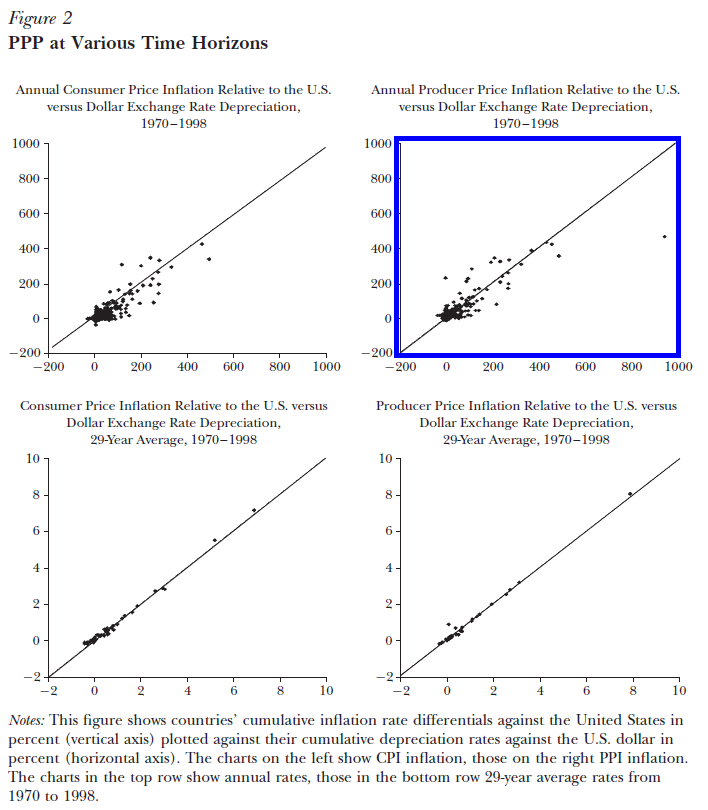
\includegraphics[width=0.75\textwidth]{Macroeconomia Internacional/APS 3 Macro Int/PPCa & PPCr.png}
    \label{fig:ppcar}
    
    \footnotesize{Fonte: Retirada do artigo Taylor & Taylor.}
    \end{figure}

A Figura~\ref{fig:ppcar} apresenta uma análise da PPC Relativa, focando na relação entre inflação relativa e depreciação da taxa de câmbio entre diferentes países em relação aos Estados Unidos ao longo de um período de várias décadas. A PPC Relativa é testada ao comparar a diferença das inflações entre países (inflação de um país menos a inflação dos EUA).

Com os resultados mostrados podemos notar que para pequenas diferenças na inflação anual, a relação entre a inflação relativa entre os países e a depreciação cambial é baixa, mostrando que a PPC Relativa não se mantém no curto prazo. No entanto, quando observados em longo prazo , os dados tendem a se aproximar mais com a previsão da PPC Relativa, sugerindo que, ajustes de curto prazo são voláteis e influenciados por fatores diversos, enquanto no longo prazo existe uma tendência de convergência entre inflação e depreciação cambial.

A PPC Relativa é mais eficinete para entender como as taxas de inflação diferencial influenciam as taxas de câmbio no longo prazo, se corrigindo para manter o equilíbrio do poder de compra entre as economias. As diferenças de curto prazo podem ser explicadas pela rigidez dos preços.

De maneira geral a PPC Absoluta quanto a PPC Relativa têm problemas para explicar as relações entre as variáveis no curto prazo, mas tendem a se verificar no longo prazo. 

\section{\textbf{Questão 3}}

\subsection{\textbf{Letra A}}
\begin{figure}[H]
    \centering
    \caption{Gráfico do Aumento da Demanda} 
    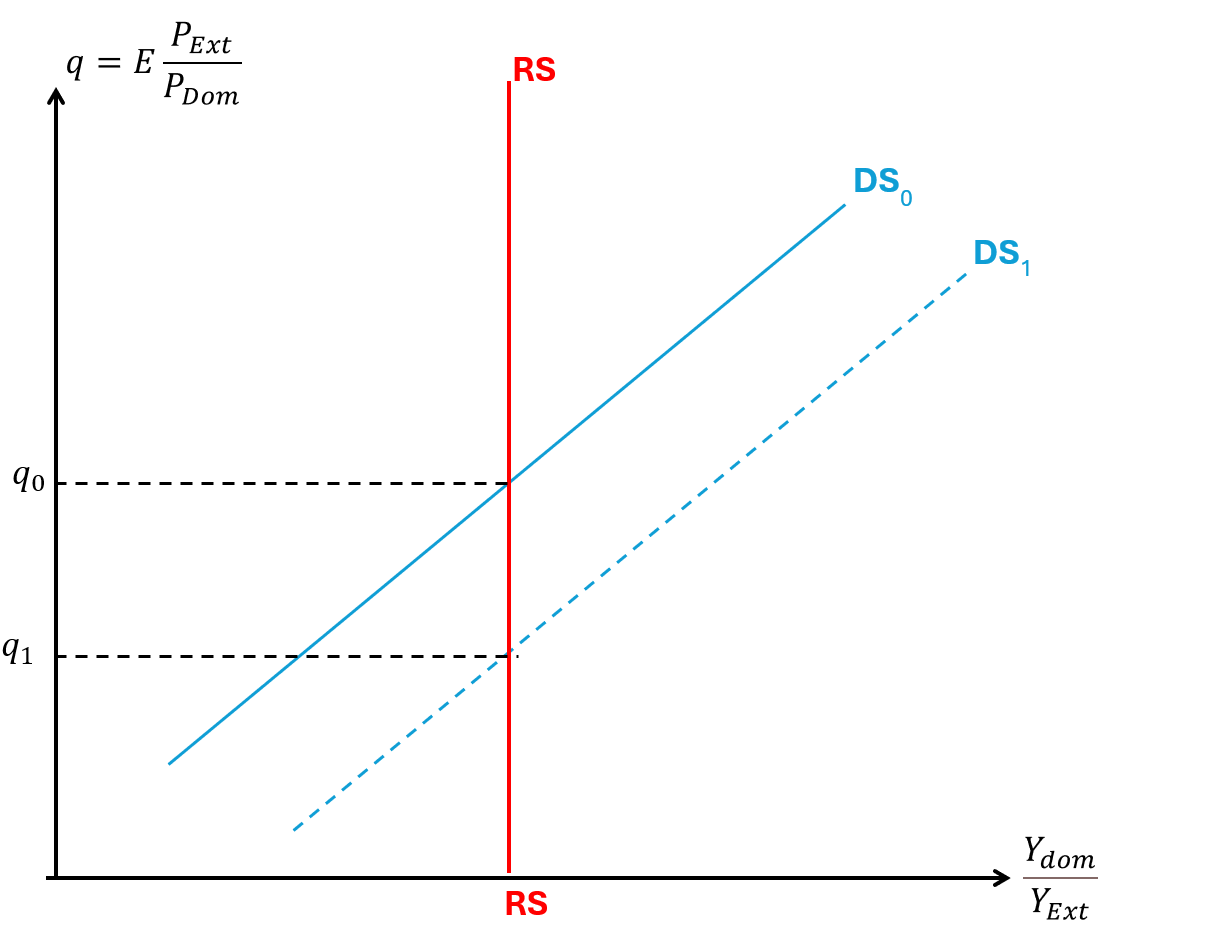
\includegraphics[width=0.75\textwidth]{Macroeconomia Internacional/APS 3 Macro Int/Gráfico do Aumento da Demanda.png}
    \label{fig:aumentodemanda}
    
    \footnotesize{Fonte: Elaborado pelos autores.}
    \end{figure}

Devido ao fluxo migratório para os países, há um choque positivo de demanda, pois novas pessoas estão dentro do mercado consumidor. Isso acaba por demandar mais produtos dada a mesma oferta, isso pode ser visto quando $DS_0$ varia para $DS_1$, dado a mesma $RS$. Esse descompasso causa um pressão sobre os preços dos produtos ingleses (ING) e faz eles aumentarem em relação aos preços dos produtos do resto do mundo (REM).

Esse aumento da demanda ING em relação ao REM causa uma apreciação do câmbio real.

\subsection{\textbf{Letra B}}
\begin{figure}[H]
    \centering
    \caption{Gráfico do Aumento da Oferta} 
    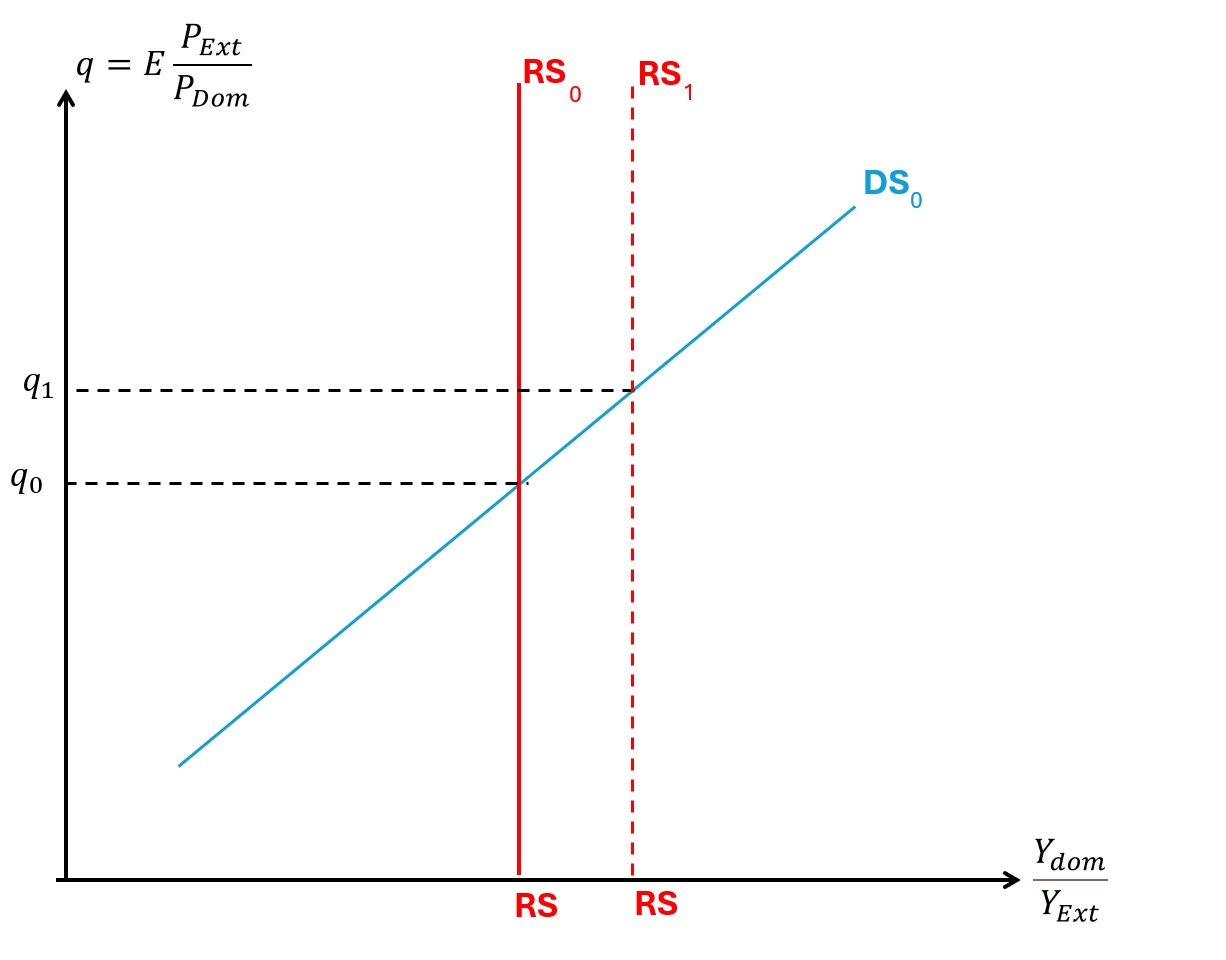
\includegraphics[width=0.75\textwidth]{Macroeconomia Internacional/APS 3 Macro Int/Gráfico do Aumento da Oferta.png}
    \label{fig:aumentooferta}
    
    \footnotesize{Fonte: Elaborado pelos autores.}
    \end{figure}

O fluxo migratório para ING gera maior disponibilidade de mão de obra, podendo aumentar a oferta.

Efeito do mercado de bens: Aumento da oferta causa diminuição dos preços relativos (Dom/Ext) causando uma desvalorização real de ING em relação à REM.

Efeito do mercado monetário: Aumento da oferta causa um aumento da demanda por moeda doméstica diminuindo o nível de preços reais de ING.

Desse modo, existe um efeito ambíguo no câmbio E(ING/REM).
\subsection{\textbf{Letra C}}

Dado as análises anteriores, seriam possíveis tanto um choque positivo na demanda quanto um choque positivo na oferta.Logo, não existe uma resposta sobre qual dos dois efeitos observados prevaleceria. 

\section{\textbf{Questão 4}}
As respostas da prova foram todos temas e intuições abordadas em aula. 

Em relação a Questão 1, sempre foi insistido pelo professor e pelo monitor "brincar" com todas em curvas, mexendo cada uma das variáveis, tanto positivamente quanto negativamente, e ver suas implicações sobre as outras curvas e explicar usando as intuições econômicas.

Sobre a Questão 2, não foi nada além da interpretação de uma parte curta de um artigo passado para a aula 18 de março, não era uma leitura pesada, ainda mais que eram apenas 6 páginas , das 6 2 eram apenas imagens de gráficos. A resposta estava inteira escrita nessas 6 páginas, era realmente uma questão dada.

Por fim a Questão 3, era uma questão extremamente simples, dado o fato da intuição para responder ela era trivial, além disso a resposta dessa questão foi dada na última aula antes da prova, ao ilustrar e explicar os gráficos de demanda e oferta relativa, essa questão apenas contextualizou usando uma situação sobre migração.

\subsection{\textbf{Perspectiva 1}}

Estudei para a prova de forma rasa, não compreendendo com profundidade a matéria e a maneira como devemos responder as questões. Também faltei com a interpretação correta do primeiro enunciado e por mais que tenha ido nas monitorias e prestado atenção nas aulas, não segui algumas dicas essenciais do monitor e do professor sobre como estudar para a matéria.
Em suma, vejo que meu desempenho foi muito pior do que o esperado por mim e pela disciplina, por mais que algumas questões lidassem com formatos básicos vistos em aula e o texto proposto pelo professor.

\subsection{\textbf{Perspectiva 2}}

Em relação aos estudos, não estive em dia com as leituras dos capítulos do livro e artigos da matéria para o melhor acompanhamento da aula. Não "brinquei" com todas as curvas em todos os sentidos e não fiz exercícios suficientes sobre a matéria para me preparar da melhor forma possível para a prova. Mas estive presente em todas as monitorias.

Em relação a minha prova, sobre a questão 1, apesar de não ter acertado a questão por inteira, me dediquei para deixar os gráficos e relações econômicos claras. Em relação a questão 2 e 3, respondi superficialmente ambas as questões com o que sabia, não quis me alongar nas questões pois não tinha total conhecimento da matéria, por motivos que citei anteriormente.

\end{document}